% Source: https://www.dropbox.com/sh/2fx6pg4ydpu9t7x/AAAdJfzvLjeym1gJwKrIWwhBa?preview=Python+Activity+05+Boolean+Expressions+-+POGIL.docx
% File: "boolean expressions.pdf"
% Access: 04-15-2022

% comment out for student version
% \ifdefined\Student\relax\else\def\Teacher{}\fi

\documentclass[12pt]{article}

\title{Activity \#5: Boolean Expressions}
\author{Lisa Olivieri}
\newcommand{\activityeditor}{Preston Carman}
\newcommand{\activitysource}{\url{https://www.dropbox.com/sh/2fx6pg4ydpu9t7x/AAAdJfzvLjeym1gJwKrIWwhBa?preview=Python+Activity+05+Boolean+Expressions+-+POGIL.docx}}
\date{Spring 2022}

\input{../../cspogil.sty}
\usepackage{tikz}

\begin{document}

\begin{center}
  \Large Activity \#5: Boolean Expressions \\[5pt]
  \large Recorder's Report\\[20pt]
  \normalsize
  \begin{tabular}{lrp{0.1in}lr}
      Manager:  & \ans{} &  & Reader: & \ans{}            \\[15pt]
      Recorder: & \ans{} &  & Driver: & \ans{}            \\[15pt]
      Date:     & \ans{} &  & Score:  & Satisfactory \hspace{10pt} /
      \hspace{10pt} Not Satisfactory
  \end{tabular}
\end{center}
\par\vskip 15pt

Record your team's answers to the key questions (marked with
\raisebox{-.3\height}{\includegraphics[width=0.5in]{../figures/key.png}})
below.
\begin{enumerate}[label=(\alph*)]
  \itemsep 1.25in
  \item Model 1, Question \#5
  \item Model 2, Question \#11
  \item Model 3, Question \#15
\end{enumerate}

\newpage
\maketitle

In this course, you will work in teams of 3--4 students to learn new concepts.
This activity will introduce you to the process of analyzing an algorithm complexity.

%\rolenames

\guide{
  \item Explain sequential, branching, and looping programming structures.
  \item Explain how relational and logical operators are used in programming.
  \item Use conditional operators with strings and numeric values.
}{
  \item Write correct Boolean expressions and compound
    expressions.\\[-5pt]
}{
No additional notes.
}

  \model{Programming Structures} \\
  \begin{center}
    \renewcommand{\arraystretch}{1.8}
    \begin{tabular}{|c|c|c|}
      \hline      
      \rowcolor{orange!20} \large Sequential Structure & \large Branching Structure & \large Looping Structure \\
      \hline
      \begin{minipage}{0.6in}
        \par\vskip 10pt
        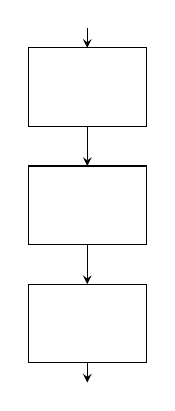
\begin{tikzpicture}
          % three boxes
          \draw (0,0) -- (1.5,0) -- (1.5,1) -- (0,1) -- (0,0);
          \draw (0,1.5) -- (1.5,1.5) -- (1.5,2.5) -- (0,2.5) -- (0,1.5);
          \draw (0,3) -- (1.5,3) -- (1.5,4) -- (0,4) -- (0,3);
          % four arrows
          \draw[-stealth] (0.75,4.25) -- (0.75,4);
          \draw[-stealth] (0.75,3) -- (0.75,2.5);
          \draw[-stealth] (0.75,1.5) -- (0.75,1);
          \draw[-stealth] (0.75,0) -- (0.75,-0.25);
        \end{tikzpicture}
        \par\vskip 4pt\ \
      \end{minipage}
      &
      \begin{minipage}{1.8in}
        \par\vskip 10pt
        \begin{tikzpicture}
          % three boxes
          \draw (1.5,0) -- (3,0) -- (3,1) -- (1.5,1) -- (1.5,0);
          \draw (0,1.75) -- (1.5,1.75) -- (1.5,2.75) -- (0,2.75) -- (0,1.75);
          \draw (3,1.75) -- (4.5,1.75) -- (4.5,2.75) -- (3,2.75) -- (3,1.75);
          % a triangle
          \draw (2.25,3) -- (3.25,3.5) -- (2.25,4) -- (1.25,3.5) -- (2.25,3);
          % and six arrows
          \draw[-stealth] (2.25,4.25) -- (2.25,4);
          \draw[-stealth] (1.25,3.5) node[above left] {\scriptsize False} -- (0.75,3.5) -- (0.75,2.75);
          \draw[-stealth] (3.25,3.5) node[above right] {\scriptsize True} -- (3.75,3.5) -- (3.75,2.75);
          \draw[-stealth] (0.75,1.75) -- (0.75,1.35) -- (2.25,1.35) -- (2.25,1);
          \draw[-stealth] (3.75,1.75) -- (3.75,1.35) -- (2.25,1.35) -- (2.25,1);
          \draw[-stealth] (2.25,0) -- (2.25,-0.25);
        \end{tikzpicture}
        \par\vskip 4pt\ \
      \end{minipage}
      &
      \begin{minipage}{1.7in}
        \centering\par\vskip 10pt
        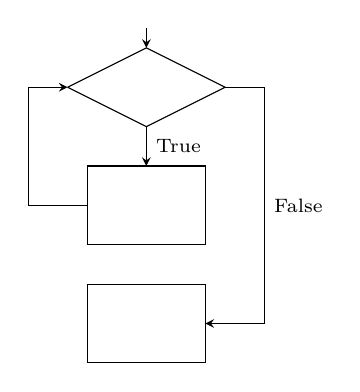
\begin{tikzpicture}
          % two rectangles
          \draw (0.25,1.5) -- (1.75,1.5) -- (1.75,2.5) -- (0.25,2.5) -- (0.25,1.5);
          \draw (0.25,0) -- (1.75,0) -- (1.75,1) -- (0.25,1) -- (0.25,0);
          % one triangle
          \draw (0,3.5) -- (1,3) -- (2,3.5) -- (1,4) -- (0,3.5);
          % five arrows
          \draw[-stealth] (1,4.25) -- (1,4);
          \draw[-stealth] (1,3) -- node[right] {\scriptsize True} (1,2.5);
          \draw[-stealth] (0.25,2) -- (-0.5,2) -- (-0.5,3.5) -- (0,3.5);
          \draw[-stealth] (2,3.5) -- (2.5,3.5) -- node[right] {\scriptsize False} (2.5,0.5) -- (1.75,0.5);
        \end{tikzpicture}
        \par\vskip 4pt\ \
      \end{minipage}
      \\
      \hline
    \end{tabular}
  \end{center}
  
  {\it\large Refer to Model 1 above as your team develops consensus answers
    to the questions below.}
    
  \quest{20 min}
      
  \Q Based only on the pictures in the model above, what do the shapes represent?
    \begin{enumerate}
      \item Rectangle
        \begin{answer}[0.4in]
          The rectangle represents a command or group of commands in a program.
        \end{answer}

      \item Diamond
        \begin{answer}[0.4in]
          The diamond represents a true/false decision that must be made.
        \end{answer}
    \end{enumerate}

  \vskip -20pt
    
  \Q Which structure best describes the types of programs you've written thus far?
    \begin{answer}[0.4in]
      The sequential structure -- our code just executes the statements in order  
    \end{answer}
    
  \Q Which structure(s) allows the programmer to create programs that decide what code to execute?
    \begin{answer}[0.4in]
      Either the branching or the looping structure.
    \end{answer}

  \newpage

  \Q A {\it relational operator} is used to test for a particular relationship between two
    values.  It returns either {\bf true}, if the relationship holds, or {\bf false}, if it 
    does not.  What relationship does each operator below test for?  If unsure, use the
    file {\tt activity05a.cpp} to try them out.
    
    \begin{enumerate}
      \itemsep 10pt
      \begin{multicols}{2}
        \item $<$  \hspace{10pt} \ans[2in]{less than}
        \item $<=$ \hspace{3pt}  \ans[2in]{less than or equal}
        \item $!=$ \hspace{5pt}  \ans[2in]{not equal}
        \item $>$  \hspace{10pt} \ans[2in]{greater than}
        \item $>=$ \hspace{3pt}  \ans[2in]{greater than or equal}
        \item $==$ \hspace{3pt}  \ans[2in]{equal to}
      \end{multicols}
    \end{enumerate}

  \vskip -30pt
    
  \Q Use the variable values below to determine the value of the
    following expressions.\key\\[-5mm]
    \begin{center}
      \begin{minipage}{3.5in}
        \begin{cpplst}
int x = 4, y = 5, z = 4;
        \end{cpplst}
      \end{minipage}
    \end{center}

    \par\vskip 10pt
    
    \begin{enumerate}
      \itemsep 10pt
      \begin{multicols}{2}
        \item \cpp{x > y}
          \hspace{14pt} \ans[0.8in]{false}
        \item \cpp{x < y}
          \hspace{14pt} \ans[0.8in]{true}
        \item \cpp{x == y}
          \hspace{9pt} \ans[0.8in]{false}
        \item \cpp{x != y}
          \hspace{10pt} \ans[0.8in]{true}
        \item \cpp{x >= z}
          \hspace{10pt} \ans[0.8in]{true}
        \item \cpp{x <= z}
          \hfill \ans[0.8in]{true}
        \item \cpp{x + y > 2 * x}
          \hfill \ans[0.8in]{true}
        \item \cpp{y * x - z != 4 \% 4 + 15}
          \hfill \ans[0.8in]{false}
        \item \cpp{pow(x,2) == abs(-16)}
          \hfill \ans[0.8in]{true}
      \end{multicols}
    \end{enumerate}

    \vskip -20pt
 
  \Q What are the two possible answers for each expression in that last question?
    \begin{answer}[0.5in]
      They can be true or false.
    \end{answer}
          
  \Q Assume the following strings have been defined. Determine the results of the following
    expressions.
    \begin{center}
      \begin{minipage}{3.5in}
        \begin{cpplst}
string word1 = "hello";
string word2 = "good-bye";
        \end{cpplst}
      \end{minipage}
    \end{center}

    \par\vskip 10pt
    
    \begin{enumerate}
      \itemsep 10pt
      \begin{multicols}{2}
        \item \cpp{word1 == word2}
          \hspace{14pt} \ans[1in]{false}
        \item \cpp{word1 != word2}
          \hspace{14pt} \ans[1in]{true}
        \item \cpp{word1 < word2}
          \hspace{14pt} \ans[1in]{false}
        \item \cpp{word1 >= word2}
          \hspace{14pt} \ans[1in]{true}
      \end{multicols}
    \end{enumerate}

  \Q How do relational operators work on strings?
    \begin{answer}[1in]
      \par
      They compare strings lexicographical.  Meaning, words that come first in the dictionary would be
      smaller than others.  To be equal, the strings must be identical.
    \end{answer}

  \newpage
  
  {\bf\large Model 2: A Truth Table} \\
  
    \begin{center}
      \renewcommand{\arraystretch}{1.4}
      \begin{tabular}{|c|c|c|c|c|}
        \hline
        \rowcolor{orange!20} Condition \#1 & Condition \#2 & Negation (NOT) & Conjunction (AND) & Disjunction (OR) \\
        \rowcolor{orange!20} \mintinline{cpp}|p| & \mintinline{cpp}|q| & \mintinline{cpp}|! p| & \mintinline{cpp}|p && q| & \mintinline{cpp}{p || q} \\
        \hline
        True & True   & False & True  & True \\
        True & False  & False & False & True \\
        False & True  & True  & False & True \\
        False & False & True  & False & False \\
        \hline
      \end{tabular}
    \end{center}

  {\it\large Refer to Model 2 above as your team develops consensus answers
    to the questions below.}
    \par\vskip 10pt

    \item The symbols \mintinline{cpp}{&&}, \mintinline{cpp}{||}, and \mintinline{cpp}{!} are called
      {\it logical operators} because they combine conditions that are either true or false to create
      new compound conditions. Given the variable definitions below, fill in the
      appropriate logical operator to produce the desired truth value.
      \begin{center}
        \begin{minipage}{3.5in}
          \begin{minted}[
            frame=lines,
            framesep=2mm,
            bgcolor=gray!15,
            baselinestretch=1.2
          ]{cpp}
  int numBooks = 40;
          \end{minted}
        \end{minipage}
      \end{center}
      \par\vskip 10pt
      \begin{enumerate}[(a)]
        \itemsep 15pt
        \item \mintinline{cpp}{(numBooks > 5)} \fillin[\mintinline{cpp}{&&} or \mintinline{cpp}{||}][1in] \mintinline{cpp}{(numBooks < 100)}
          -- this should be {\bf true}.
        \item \mintinline{cpp}{(numBooks < 5)} \fillin[\mintinline{cpp}{||}][1in] \mintinline{cpp}{(numBooks > 20)}
          -- this should be {\bf true}.
        \item \fillin[\mintinline{cpp}{!}][1in]\mintinline{cpp}{ (numBooks * 10 == 400)} 
          -- this should be {\bf false}.
      \end{enumerate}

    \item A {\it Boolean Expression} is an expression that uses relational operators and/or logical operators together with
      variables, literal values, and the {\it Boolean} values ``true'' and ``false''. Translate the following Boolean expressions 
      into an English statement.  The first one is done for you.
      \par\vskip 15pt
      \begin{enumerate}[(a)]
        \itemsep 15pt
        \item \mintinline{cpp}{(x == 2) && (y > 3)}
          \hfill\underline{\hspace{8pt}The variable x equals two and the variable y is bigger than three.\hspace{9pt}}
        \item \mintinline{cpp}{(x != 4) || (y <= 7)}
          \hfill\fillin[x is not equal to four or y is less than or equal to seven.][4.2in]
        \item \mintinline{cpp}{(x >= 2) && (x <= 10)}
          \hfill\fillin[x is between two and 10 inclusively][4.2in]
        \item \mintinline{cpp}{!((x == 2) && (y == 1))}
          \hfill\fillin[it is not the case that x is two and y is one.][4.2in]
      \end{enumerate}
      \par\vskip -40pt\ \
      
    \item Write a Boolean Expression for each English statement.\key\\[-2.5mm]
      \par\vskip 10pt

      \begin{enumerate}[(a)]
        \itemsep 15pt
        \item The string {\tt name} is not equal to ``Jane''.                     \hfill \fillin[\mintinline{cpp}{word != "Jane"}][2in]
        \item The value of $x$ is twice that of $y$ or $y$ is less than ten.      \hfill \fillin[\mintinline{cpp}{(x==2*y)||(y<=10)}][2in]
        \item The value of $z$ is between 0 and 5 excluding endpoints.            \hfill \fillin[\mintinline{cpp}{(z>0)&&(z<5)}][2in]
        \item It is not the case that $w$ is between 0 and 5 including endpoints. \hfill \fillin[\mintinline{cpp}{!((w>=0)&&(w<=5))}][2in]
      \end{enumerate}
  \newpage
  \model{A C++ Program} \\
  \begin{center}
    \small
    \begin{minipage}{5.5in}
      \begin{cprlst}[
        frame=lines,
        framesep=2mm,
        bgcolor=gray!15,
        baselinestretch=1.2,
        linenos
      ]{cpp}
#include <iostream>
using namespace std;

int main() {
  float originalPrice, salePrice;
  cout << "Enter the original cost of the item: ";
  cin >> originalPrice;
  cout << "Enter the sale price: ";
  cin >> salePrice;
  int percentOff = ((originalPrice - salePrice)/originalPrice) * 100;
  cout << "Percent off: " << percentOff << "%" << endl;
  if (percentOff >= 50) {
    cout << "You found a great deal!" << endl;
  }
}      
      \end{cprlst}
    \end{minipage}
  \end{center}
  \TPMargin{5pt}
  
  
  {\it\large Refer to Model 1 above as your team develops consensus answers
    to the questions below.}
    \par\vskip 10pt
    
  \begin{enumerate}
    \itemsep 20pt
    
    \Q You will find this program in {\tt activity06a.cpp}.  Run it with various
      original cost and sale prices and then answer the questions below.
      \begin{enumerate}[(a)]
        \item What do lines 6 and 7 do?%\ifprintanswers\par\vskip -20pt\null\fi
          \begin{answer}[0.4in]
            They prompt for and store the original price in the {\tt originalPrice} variable.
          \end{answer}%\ifprintanswers\par\vskip -20pt\null\fi
        \item What do lines 8 and 9 do?%\ifprintanswers\par\vskip -20pt\null\fi
          \begin{answer}[0.4in]
            They prompt for and store the sale price in the {\tt salePrice} variable.
          \end{answer}%\ifprintanswers\par\vskip -20pt\null\fi
        \item What do lines 10 and 11 do?%\ifprintanswers\par\vskip -20pt\null\fi
          \begin{answer}[0.4in]
            They compute the percent price reduction and print it out.
          \end{answer}%\ifprintanswers\par\vskip -20pt\null\fi
        \item What do lines 12-14 do?%\ifprintanswers\par\vskip -20pt\null\fi
          \begin{answer}[0.4in]
            They print out ``You found a great deal!'' if the savings was
            50\% or more.
          \end{answer}%\ifprintanswers\par\vskip -20pt\null\fi
      \end{enumerate}
      
    \Q Revise the program in model 1 so that right after printing ``You found a great
      deal!'' it prints ``Congratulations!'' if the percent savings was 50\% or more.  Use a
      separate {\tt cout} statement to do this and make note of what you did below.
      \begin{answer}[1in]
        We added the command:\vskip -20pt\null
        \begin{center}
          \begin{minipage}{3.5in}
            \begin{cprlst}[
              frame=lines,
              framesep=2mm,
              bgcolor=gray!15,
              baselinestretch=1.2,
              linenos
            ]{cpp}
    cout << "Congratulations!" << endl;
            \end{cprlst}
          \end{minipage}
        \end{center}\vskip -15pt\null
        right below line 13.
      \end{answer}
      % \ifprintanswers\vskip -30pt\null\fi
      
    \Q Revise the code further so that it prints ``Done!'' when the program is
      complete, no matter what the percent off is.  Again, use a separate {\tt cout}
      statement and describe how the placement of this line of code differs from the
      placement of the code you added above.
      \begin{answer}[1in]
        We added the line of code\vskip -20pt\null
        \begin{center}
          \begin{minipage}{3.5in}
            \begin{cprlst}[
              frame=lines,
              framesep=2mm,
              bgcolor=gray!15,
              baselinestretch=1.2,
              linenos
            ]{cpp}
  cout << "Done!" << endl;
            \end{cprlst}
          \end{minipage}
        \end{center}\vskip -15pt\null
        right below the curly brace on line 14 of the original program (line 15 after or
        modification above.
      \end{answer}
      % \ifprintanswers\vskip -40pt\null\fi

    \item What happens if you remove the open curly brace (\cpp{\{}) from the
      end of line 12 and the close\key\\[-2.5mm] curly brace (\cpp{\}}) from line 14 (15 in
      your modified program)?  Explain why this happens.
      
      \begin{answer}[1in]
        \par
        If we remove these curly braces, the program always prints ``Congratulations!'',
        regardless of what the percent savings is.  This is because the {\tt if} statement
        only  applies to the next statement or block of statements.  Removing the curly brace
        makes it only apply to line 13.
      \end{answer}
      
  
    
\end{document}
